\subsection{Effect of Memory Bandwidth Throttling}

In this subsection, we examine the DNN workload's memory bandwidth
sensitivity and the effect of memory bandwidth throttling in providing
isolation. For the experiments, we use MemGuard\cite{Yun2013}, which 
can limit the amount of memory bandwidth each core receives. MemGuard
operates periodically, at an 1ms interval, and uses hardware
performance counters to throttle cores if they exceed their given
bandwidth budgets within each regulation period (i.e., 1ms) by
scheduling high-priority idle kernel threads.

In the first experiment, we measure the performance of the DNN model
running on a single core, Core 0, first w/o using MemGuard and then w/
using MemGuard while varying the core's bandwidth throttling parameter
from 500 MB/s down to 100 MB/s.

\begin{figure}[h]
  \centering
  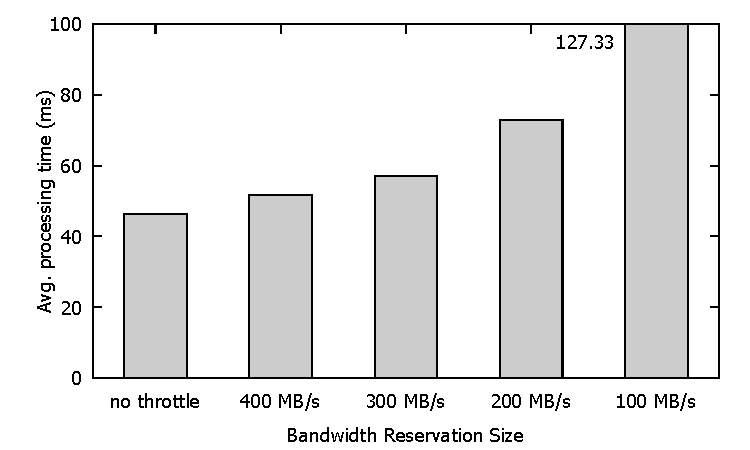
\includegraphics[width=.45\textwidth]{figs/memguard_multicore}
  \caption{ Memory bandwidth sensitivity of the control loop 
execution time. }
  \label{fig:memguard_multicore}
\end{figure}

Figure \ref{fig:memguard_multicore} shows the result. When the DNN
model executing core is throttled at 400 MB/s or more, performance of
the model is largely the same as the non-throttled case. However, as
we decreate the assigned memory badnwdith below 300 MB/s, we start to
observe noticably decreases in the model's performance. In other
words, the DNN model is sensitive to memory bandwidth and that it
requires 400 MB/s or more bandwidth should be given to ensure ideal
performance.

In the next experiment, we again repeat the experiment in
Section~\ref{sec:eval-memhog}---i.e., co-scheduling the DNN model and
three Bandwidth (BwRead or BwWrite) instances---but this time we
throttle the cores that execute the co-runners using MemGuard by 
varying their bandwidth budgets to see ther impact in the DNN model's
performance. 

\begin{figure}[h]
  \centering
  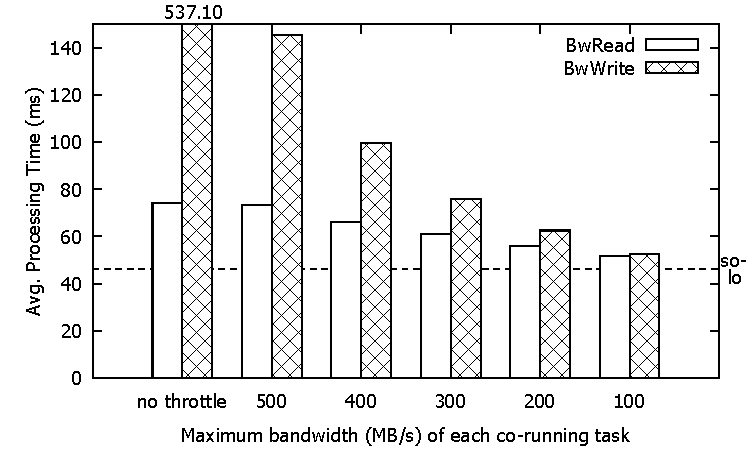
\includegraphics[width=.45\textwidth]{figs/memguard_bandwidth}
  \caption{Timing impact of co-scheduling memory intensive
co-runners when memory bandwidth throttling is enabled. }
  \label{fig:memguard_bandwidth}
\end{figure}

Figures \ref{fig:memguard_bandwidth} shows the result.
Note that, in case of BwWrite co-runners, we have assigned half the
bandwidth budget because MemGuard currently only account L2 refills
but not write-backs, which effectively allow twice the allocated
memory bandwidth budget. Regardless, the result clearly shows that
limiting co-runners's memory bandwidth is effective in protecting the
DNN model's performance.

In summary, we find that the DNN inferencing workload is sensitive to
memory bandwidth and that memory bandwidth throttling is effective in
improving performance isolation of the DNN workload.

%% \begin{figure}[h]
%%   \centering
%%   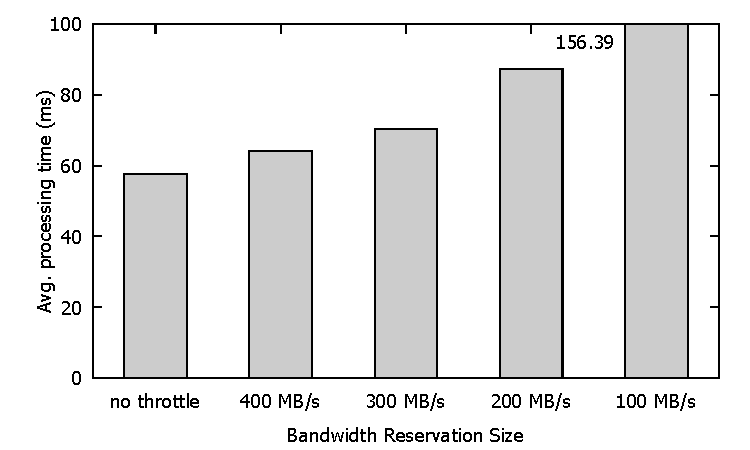
\includegraphics[width=.45\textwidth]{figs/memguard_multimodel}
%%   \caption{Timing impact of co-scheduling multiple DNNs when memory
%% bandwidth throttling is enabled. }
%%   \label{fig:memguard_multimodel}
%% \end{figure}

%% We also test the effects of memory bandwidth throttling in the case 
%% of multiple models running concurrently on the Pi 3 by rerunning the 
%% 4Nx1C experiment. We use the same memory bandwidth reservation sizes 
%% from the previous experiment. The results can be seen in Figure
%% \ref{fig:memguard_multimodel}. Once again, the performance of the 
%% models are affected by the amount of memory bandwidth that is 
%% available to the Pi 3's cores during each period, meaning that they 
%% are all memory dependent.

%% \begin{figure}[h]
%%   \centering
%%   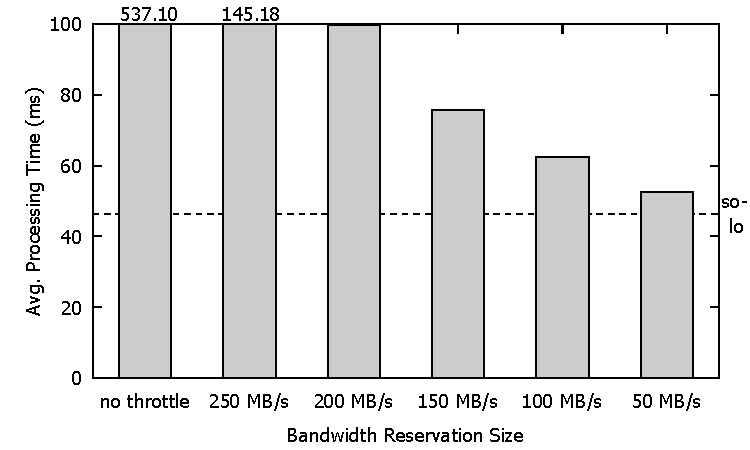
\includegraphics[width=.45\textwidth]{figs/memguard_bwwrite}
%%   \caption{Timing impact of co-scheduling memory intensive write
%% co-runners when memory bandwidth throttling is enabled. }
%%   \label{fig:memguard_bwwrite}
%% \end{figure}


%% In the case of one co-runner, the performance of the model remains 
%% constant even as the reservation sizes are decreased, however, it 
%% still improves compared to when throttling wasn't enabled. 
%% In both cases, when the co-runners were given a minimal reservation size,
%% the performance of the model was much closer to its solo execution time.
%% This is especially noteworthy when write co-runners were present, as the 
%% model didn't suffer the same 11.6X slowdown that was seen without
%% bandwidth throttling enabled. 
%% %% When memory intensive Bandwidth benchmarks were present, model performance
%% %% improved, to a notable extent, through the use of memory bandwidth 
%% %% throttling on the co-runners. 
%% Since this would not be the case if the 
%% model was memory insensitive, we find that the model is memory 
%% dependent in the presence of co-runners.

%% Based on all of the memory bandwidth throttling experiments 
%% performed, it is evident that the shared DRAM memory is important for
%% the DNN model. When a single model was run, its 
%% performance decreased as less memory bandwidth was 
%% made available to it. Furthermore, when the bandwidths of memory 
%% intensive read and write co-runners were limited, the performance of 
%% the model improved. As such, we conclude that the model is dependent on the 
%% shared DRAM memory.
